\chapter{Ambiente e strumenti}
\section{Il debugger - GDB e QEMU}
\subsection{Quick emulator - QEMU}
QEMU é un emulatore open-source, permette di emulare l'architettura di un processore. Permette quindi l'utilizzo di vari sistemi operativi ad un livello di virtualizzazzione Kernel-Based (Kernel Vitual Machine - KVM) con il beneficio di prestazioni vicine all'hardware. Per il nostro utilizzo QEMU emula un sistema x86-64. 
\subsection{GNU Debugger - GDB}
GNU Debugger (GDB) è un debugger portatile, permette quindi di testare e effettuare il debug di programmi. Eseguire il programma in questo ambiente controllato permette al programmatore di tenere traccia dell'esecuzione e monitorare le risorse al fine di individuare un eventuale malfunzionamento nel codice. Per la realizzaione dell'estensione utilizzeremo la funzione di debug remoto per connetterci ad un socket di sistema utilizzato da QEMU per il debug. GDB utilizza delle chiamate di sistema chiamate \codeword{process trace} (\codeword{ptrace}). 

\subsubsection{Breakpoints}
Un breakpoint permette al programma in esecuzione all'interno di un debugger di interrompere il flusso in un determinato punto. Si realizzano sostituendo all'istruzione, alla quale si vuole fermare l'esecuzione, una speciale istruzione la quale solitamente invia un segnale SIGTRAP, il quale verrà catturato dal debugger. Il procedimento di sostituzione è eseguito dal debugger stesso prima di avviare l'esecuzione, nel caso di GDB il programmatore deve eseguire il comando \codeword{break [arg]} dove l'argomento può essere la specifica linea di codice o un simbolo. 

\subsubsection{Continue e Stop}
Tramite i comandi \codeword{continue} e \codeword{stop} possiamo rispettivamente, a seguito di un interruzione, continuare la normale esecuzione del codice oppure interrompere l'esecuzione del programma.

\subsubsection{Step Over}
Permette di proseguire alla prossima istruzione senza entrare nei componenti interni delll'istruzione a cui siamo fermi attualmente.

\subsubsection{Step Into}
Rende possibile seguire il codice riga-per-riga entrando anche nei componenti interni e subroutine.

\subsubsection{Step Out}
Quando all'interno di una subroutine e si vuole risalire al chiamante, il comando \codeword{stepOut} permette di far continuare l'esecuzione fino a ritornare all'istruzione successiva del chiamante.

\subsubsection{Analisi delle variabili}
Durante l'esecuzione vi può essere la necessità di osservare come il valore o il tipo di una variabile cambi. Inoltre é possibile cambiare il valore delle variabili ad esecuzione avviata.

\subsubsection{Call Stack}
Il call stack, o program stack, é una struttura che permette di raccogliere informazioni su tutte le subroutine di un programma in esecuzione. Tale struttura é utile per tenere traccia di quale routine ha il controllo del flusso di istruzioni e a chi deve restituire tale controllo al termine della propria esecuzione.

\subsubsection{Comandi personalizzati}
Ulteriore funzione di GDB è la possibilità di estendere le funzionalità, tramite script in python, come la creazione di comandi personalizzati.

\section{L'architettura del debugger di VS Code}
Tipicamente se si vuole creare un debugger e la sua interfaccia grafica bisogna implementare l'intera applicazione. Microsoft ha realizzato un protocollo che permette di comunicare con i debugger: il Debug Adapter Protocol (DAP). VSCode, o altri applicativi, tramite il DAP si interfaccia non direttamente al debugger ma a un attore intermedio, il Debug Adapter (DA) il quale si occupa di trasformare le richieste dell'applicazione in comandi per il debugger di destinazione.

\begin{figure}[H]
    \centering
    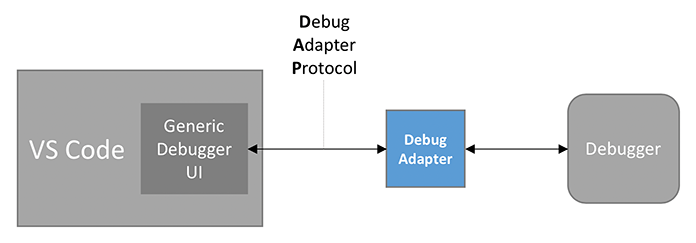
\includegraphics[width=0.7\columnwidth]{images/debug-arch1.png}
    \caption{DAP e DP}
    \label{fig:dap e dp}
\end{figure}

Rende possibile quindi la realizzazione di una generica interfaccia di debug la quale poi si occupa di comunicare con uno o piú DP. Inoltre i Debug Adapters possono essere riutilizzati in diversi ambienti di sviluppo, eliminando la necessitá di crearne uno specifico per ogni esigenza. 

\begin{figure}[H]
    \centering
    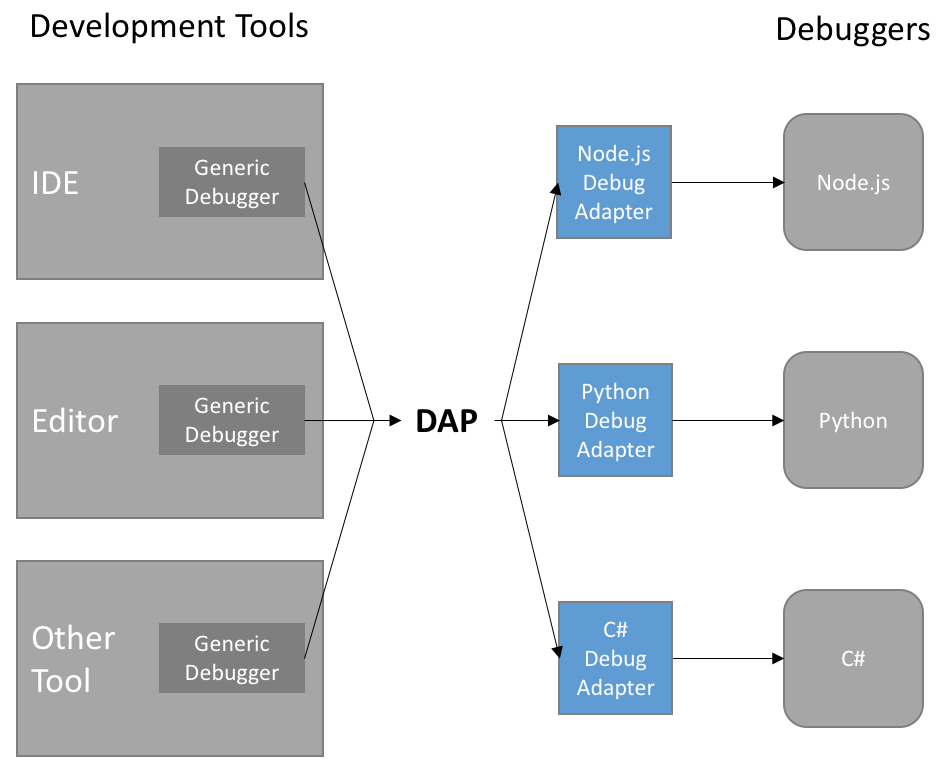
\includegraphics[width=0.7\columnwidth]{images/with-DAP.png}
    \caption{Ambienti di sviluppo multipli}
    \label{fig:Ambienti di sviluppo multipli}
\end{figure}

\subsection{Debug Adapter Protocol e Debug Adapter}

Analizziamo come avviene la connessione e scambio di messaggi tra l'applicativo e il debugger. Gli strumenti di sviluppo possono interagire con il Debug Adapter in due modi:
\begin{itemize}
    \item {
        Modalità a singola sessione: l'applicazione avvia una sessione di debug singola e comunica attraverso \codeword{stdin} e \codeword{stdout}. Alla fine della sessione, il Debug Adapter viene terminato
    }
    \item {
        Modalità a sessioni multiple: l'applicazione di debug si connette a un debugger già avviato in precendenza e si disconnette al termine della sessione.
    }
\end{itemize}


Il DAP supporta molte funzionalità, ciascuna rappresentata da una "capacità". Quando inizia una sessione di debug, lo strumento di sviluppo invia una richiesta di inizializzazione per capite le funzionalità dell'adattatore. Dopo l'inizializzazione, il Debug Adapter è pronto per accettare richieste di avvio o collegamento.
\subsubsection*{Breakpoint}
Lo strumento di sviluppo gestisce i breakpoint inviando le informazioni di configurazione all'adattatore prima dell'esecuzione del programma. Quando il programma si ferma, l'adattatore, solitamente, invia un evento di stop con il motivo e l'id del thread. Lo strumento di sviluppo richiede i thread e lo stacktrace, e tramite essi risalire alle variabili.

\subsubsection*{Inizio della sessione di debug}
Dopo aver stabilito una connessione, lo strumento di sviluppo comunica con l'adattatore tramite il protocollo di base. Il protocollo di base é implementato tramite lo scambio di messaggi composti da un'intestazione e un contenuto, chiamati \codeword{ProtocolMessage}. 

\begin{figure}[H]    
    \centering
    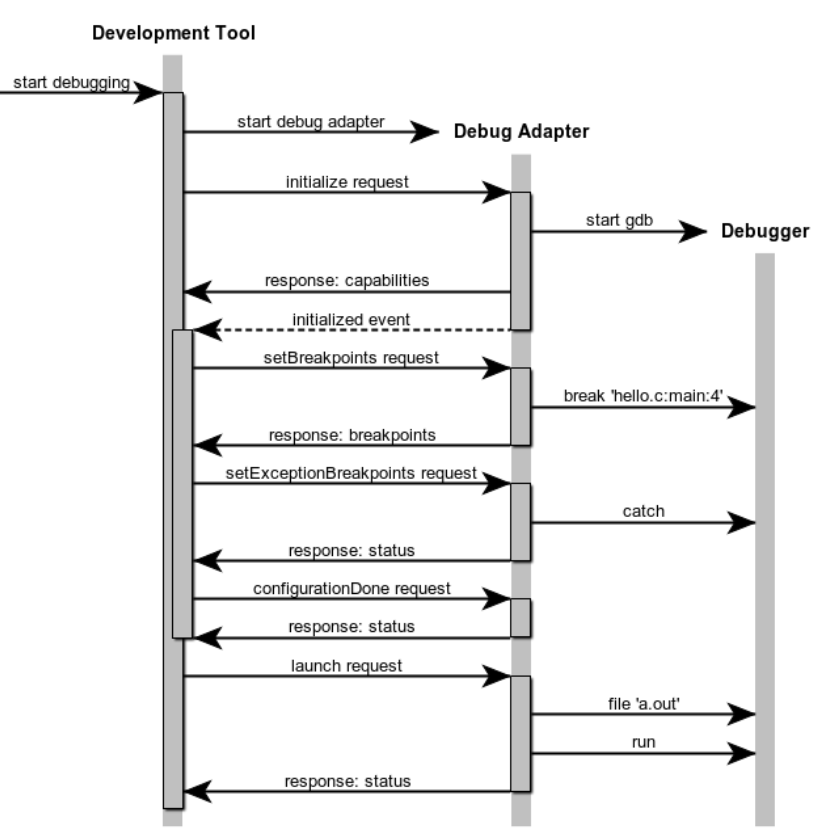
\includegraphics[width=0.7\columnwidth]{images/init-launch.png}
    \caption{Esempio di avvio di una sessione di debug\cite{DAP}}
\end{figure}

Quando inizia una sessione di debug, lo strumento di sviluppo deve comunicare con l'adattatore di debug che implementa il Protocollo di Adattatore di Debug (Debug Adapter Protocol, DAP). Il protocollo di base é implementato tramite lo scambio di messaggi composti da un'intestazione e un contenuto, chiamati \codeword{ProtocolMessage}. 
\begin{figure}[H]
    \lstinputlisting[language=JavaScript]{code/protocolMessage.txt}
    \caption{ProtocolMessage\cite{DAPmessage}}
\end{figure}

\subsubsection*{Termine della sessione di debug}

Il processo per terminare la sessione è diverso a seconda di come si é avviata la sessione, "avviato" o "agganciata":

\begin{itemize}
    \item {
        debugger "avviato": se il Debug Adapter implementa la richiesta di interruzione, allora la sessione viene terminata correttamente. Se non dovesse essere supportata la sessione continua a essere attiva fino a quando il debugger stesso non invia il comando di terminazione forzata
    }
    \item {
        debugger "agganciato": l'applicazione di debug  invia una richiesta di disconnessione al Debug Adapter. Questo permette al debugger di cessare la connessione con l'applicativo e continuare l'esecuzione
    }
\end{itemize}

se la sessione di debug termina, e il Debug Adapter è opportunamente configurato, un messaggio di corretta terminazione di sessione viene inviato all'applicazione di debug del programmatore.

\begin{figure}[H]    
    \centering
    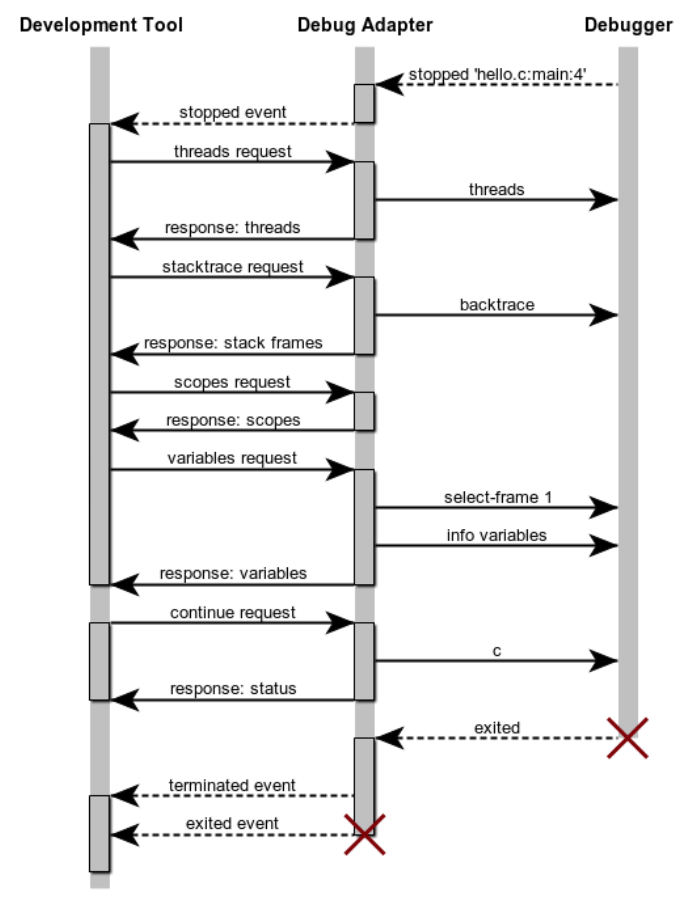
\includegraphics[width=0.7\columnwidth]{images/stop-continue-terminate.png}
    \caption{Esempio terminazione di una sessione di debug\cite{DAP}}
\end{figure}

\subsection{Logpoints}
I logpoint sono una variante dei breakpoint. Permettono, senza interrompere l'esecuzione, di controllare il valore di una o più variabili e mostrando il risultato nell console di debug di VSCode. Sono molto utili per evitare aggiungere codice di log all'interno del programma.

\section{Webview di VS Code}

VSCode mette a disposizione la possibilitá di creare nuove schede nelle quali un utente può visializzare contenuti personalizzati. Le webview sono molto simili a \codeword{iframe} e sono capaci di renderizzare ualsiasi contenuto HTML e scambio di informazioni tra la webview e VSCode. 

\begin{figure}[H]
    \centering
    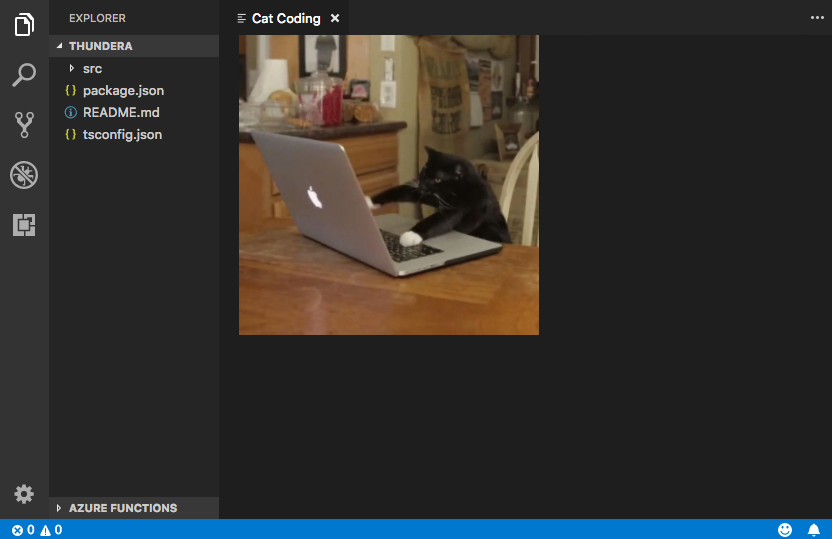
\includegraphics[width=0.7\columnwidth]{images/cat_coding.png}
    \caption{Esempio di una webview in VSCode}
    \label{fig:webcat}
\end{figure}
